\documentclass[12pt, a4paper]{article}
\usepackage[utf8]{inputenc}
\usepackage[brazilian]{babel} % Hifenização e dicionário
\usepackage[left=3.00cm, right=2.00cm, top=3.00cm, bottom=2.00cm]{geometry}
\usepackage{enumitem} % Para itemsep etc
\usepackage{longtable} % Dependência do longtabu
\usepackage{tabu} % Para melhor criação de tabelas
\usepackage{listings} % Para códigos
\usepackage{lstautogobble} % Códigos indentados corretamente
\usepackage{color} % Para coloração de códigos
\usepackage{zi4} % Para fonte de códigos
\usepackage{parskip} % Linha em branco entre parágrafos em vez de recuo
\usepackage{graphicx}
\usepackage{float}
\usepackage{verbatim}
\usepackage[autostyle]{csquotes}
\usepackage[breaklinks]{hyperref}


\usepackage{listings}
\lstset{
    autogobble,
    columns=fullflexible,
    showspaces=false,
    keepspaces=true,
    showtabs=true,
    breaklines=true,
    showstringspaces=false,
    breakatwhitespace=true,
    escapeinside={(*@}{@*)},
    commentstyle=\color{greencomments},
    keywordstyle=\color{bluekeywords},
    stringstyle=\color{redstrings},
    numberstyle=\color{graynumbers},
    basicstyle=\ttfamily\footnotesize,
    frame=l,
    framesep=12pt,
    xleftmargin=12pt,
    tabsize=4,
    captionpos=b,
}

\newcommand{\ic}[1]{\textbf{\lstinline{#1}}}

\DeclareGraphicsExtensions{.pdf, .png}

\begin{document}

\begin{center}
    \textsc{Universidade Federal do Rio Grande do Norte} \\
    \textsc{Departamento de Informática e Matemática Aplicada}
\end{center}

\bigskip

\begin{tabular}{@{}ll@{}}
    \emph{Disciplina:} & DIM0611 --- Compiladores \\
    \emph{Docente:}    & Martin Alejandro Musicante \\
    \emph{Discente:}   & Felipe Cortez de Sá \\
\end{tabular}

\bigskip

\begin{center}
\large \textbf{Parsers preditivos}
\end{center}

O cálculo dos conjuntos \ic{FIRST}, \ic{FOLLOW} e da tabela de predição foram
feitos através das ferramentas \cite{jsmachines} e \cite{hackingoff},
usando como entrada a gramática desenvolvida na primeira atividade.

Os tokens são acessados através da função \ic{yylex()}, inclusa no arquivo
gerado pelo lexer desenvolvido anteriormente.

Para simplificar o entendimento do código, cada terminal e não terminal tem um
macro correspondente (prefixo \ic{T_} para terminais e \ic{NT_} para não
terminais) substituído por um inteiro ao compilar. Os macros estão definidos no
arquivo \ic{lex}. Há uma função \ic{get\_token(char tok)} que recebe o inteiro
associado ao token e devolve a string correspondente para facilitar a
depuração.

\section{Parser por tabela}
Foi implementada uma pilha que armazena símbolos (codificados por \ic{chars}).
O resultado do processo de parsing é salvo num arquivo \ic{.dot} e pode ser
visualizado através do programa \ic{graphviz} \cite{graphviz} com o comando \ic{graphviz
graph.dot -Tpdf -o graph.pdf}.

As produções estão definidas na matriz \ic{r} como cadeias de caracteres, em
que cada caractere corresponde a um símbolo terminal ou não-terminal. A matriz
\ic{rules2}, gerada pela ferramenta \cite{hackingoff}, contém os índices das
regras definidas em \ic{r} (com as regras de código 89 e 90 indicando erros),
onde cada coluna corresponde a um terminal e cada linha corresponde a um
não-terminal. A ordem desses símbolos nas linhas e colunas seguem a ordem em
que aparecem os terminais na tabela do conjunto \ic{FIRST} e os não terminais
que aparecem no conjunto \ic{FOLLOW} na ferramenta. Tendo isso em vista, os
macros definidos seguem essa ordem para a numeração.

\begin{figure}[h]
    \centering
    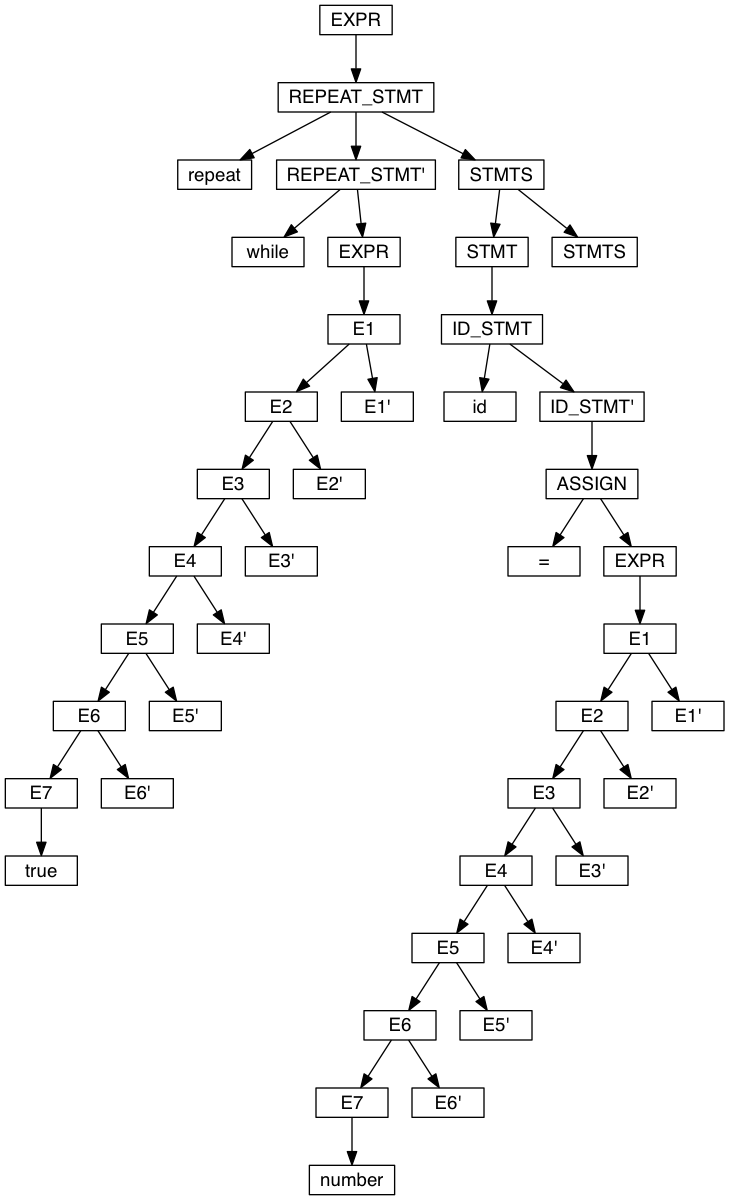
\includegraphics[width=0.40\textwidth]{graph}
    \caption{Árvore gerada pelo \ic{graphviz}}
    \label{fig:graph_1}
\end{figure}

\section{Parser recursivo}
Foi utilizado o algoritmo apresentado por Appel \cite{modern} na seção 3.2.

Para cada não-terminal da gramática foi implementada uma função recursiva que,
com base no conjunto \ic{FIRST}, determina a regra a ser seguida, chamando as
funcões recursivas associadas aos não-terminais da produção e a função
\ic{eat()} para os símbolos terminais. Para produções que geram $ \epsilon $, a
função retorna sem chamadas adicionais. Para cada \ic{switch}, há um caso
\ic{default} que chama uma função \ic{error()} caso o token sendo lido não
esteja no conjunto \ic{FIRST}. O token atual é armazenado numa
variável global \ic{current_tok} para não haver necessidade de passar ponteiros
para todas as funções.

\begin{thebibliography}{9}

\bibitem{jsmachines}
\textit{JS Machines --- LL(1) parser generator}. \\
\url{http://jsmachines.sourceforge.net/machines/ll1.html}

\bibitem{hackingoff}
\textit{HackingOff --- LL(1) parser generator}. \\
\url{http://hackingoff.com/compilers/ll-1-parser-generator#ll-1-parsing-table}

\bibitem{graphviz}
\textit{Graphviz --- Graph Visualization Software}. \\
\url{http://www.graphviz.org/}

\bibitem{modern}
Andrew W. Appel.
\textit{Modern compiler implementation in ML}.
Cambridge University Press, 1998.

\end{thebibliography}

\end{document}
